% This file was created with tikzplotlib v0.10.1.
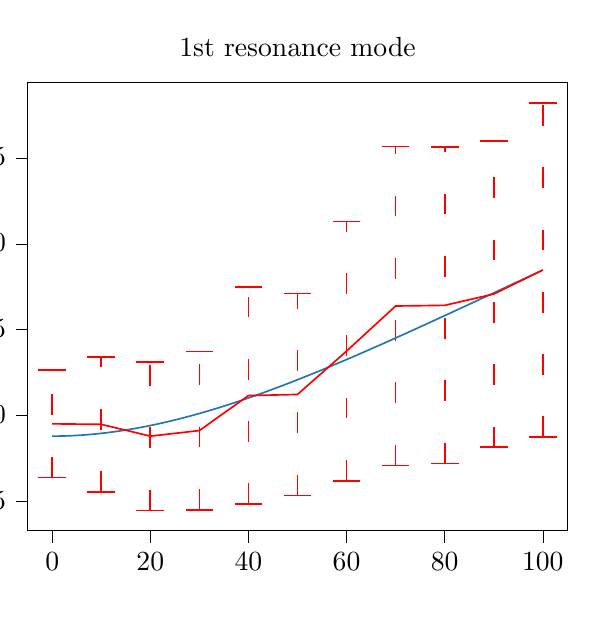
\begin{tikzpicture}[
trim axis left,
trim axis right
]

\definecolor{darkgray176}{RGB}{176,176,176}
\definecolor{steelblue31119180}{RGB}{31,119,180}

\begin{axis}[
tick align=outside,
tick pos=left,
title={1st resonance mode},
x grid style={darkgray176},
xlabel={\si{\micro\meter}},
xmin=-5, xmax=105,
xtick style={color=black},
y grid style={darkgray176},
ylabel={average \si{\decibel}},
ymin=-76.7137982896193, ymax=-50.601562414498,
ytick style={color=black}
]
\path [draw=red, semithick, dash pattern=on 7.5pt off 15pt]
(axis cs:0,-73.6091708968622)
--(axis cs:0,-67.3548291031378);

\path [draw=red, semithick, dash pattern=on 7.5pt off 15pt]
(axis cs:10,-74.4430953666532)
--(axis cs:10,-66.5819955424377);

\path [draw=red, semithick, dash pattern=on 7.5pt off 15pt]
(axis cs:20,-75.5268784771138)
--(axis cs:20,-66.8720306137953);

\path [draw=red, semithick, dash pattern=on 7.5pt off 15pt]
(axis cs:30,-75.483075371379)
--(axis cs:30,-66.2663791740755);

\path [draw=red, semithick, dash pattern=on 7.5pt off 15pt]
(axis cs:40,-75.1560033484002)
--(axis cs:40,-62.5189057425088);

\path [draw=red, semithick, dash pattern=on 7.5pt off 15pt]
(axis cs:50,-74.6554287278903)
--(axis cs:50,-62.888207635746);

\path [draw=red, semithick, dash pattern=on 7.5pt off 15pt]
(axis cs:60,-73.798410708432)
--(axis cs:60,-58.6964983824771);

\path [draw=red, semithick, dash pattern=on 7.5pt off 15pt]
(axis cs:70,-72.904254858874)
--(axis cs:70,-54.3364724138533);

\path [draw=red, semithick, dash pattern=on 7.5pt off 15pt]
(axis cs:80,-72.7877090162907)
--(axis cs:80,-54.375563710982);

\path [draw=red, semithick, dash pattern=on 7.5pt off 15pt]
(axis cs:90,-71.8486955411609)
--(axis cs:90,-53.9985771861119);

\path [draw=red, semithick, dash pattern=on 7.5pt off 15pt]
(axis cs:100,-71.2616995911783)
--(axis cs:100,-51.7884822270035);

\addplot [semithick, red, mark=-, mark size=5, mark options={solid}, only marks]
table {%
0 -73.6091708968622
10 -74.4430953666532
20 -75.5268784771138
30 -75.483075371379
40 -75.1560033484002
50 -74.6554287278903
60 -73.798410708432
70 -72.904254858874
80 -72.7877090162907
90 -71.8486955411609
100 -71.2616995911783
};
\addplot [semithick, red, mark=-, mark size=5, mark options={solid}, only marks]
table {%
0 -67.3548291031378
10 -66.5819955424377
20 -66.8720306137953
30 -66.2663791740755
40 -62.5189057425088
50 -62.888207635746
60 -58.6964983824771
70 -54.3364724138533
80 -54.375563710982
90 -53.9985771861119
100 -51.7884822270035
};
\addplot [semithick, steelblue31119180]
table {%
0 -71.1994545454545
1.01010101010101 -71.1977272951728
2.02020202020202 -71.1925777145276
3.03030303030303 -71.1840540585421
4.04040404040404 -71.1722045812819
5.05050505050505 -71.1570775347594
6.06060606060606 -71.1387211674097
7.07070707070707 -71.117183722145
8.08080808080808 -71.0925134339931
9.09090909090909 -71.064758527327
10.1010101010101 -71.0339672126906
11.1111111111111 -71.000187683228
12.1212121212121 -70.9634681107219
13.1313131313131 -70.9238566412475
14.1414141414141 -70.8814013904474
15.1515151515152 -70.8361504384356
16.1616161616162 -70.7881518243341
17.1717171717172 -70.7374535404508
18.1818181818182 -70.6841035261031
19.1919191919192 -70.6281496610945
20.2020202020202 -70.5696397588498
21.2121212121212 -70.5086215592147
22.2222222222222 -70.4451427209277
23.2323232323232 -70.3792508137676
24.2424242424242 -70.3109933103858
25.2525252525253 -70.2404175778268
26.2626262626263 -70.1675708687454
27.2727272727273 -70.0925003123243
28.2828282828283 -70.0152529049009
29.2929292929293 -69.9358755003065
30.3030303030303 -69.8544147999265
31.3131313131313 -69.7709173424852
32.3232323232323 -69.6854294935642
33.3333333333333 -69.5979974348568
34.3434343434343 -69.5086671531679
35.3535353535354 -69.4174844291625
36.3636363636364 -69.3244948258702
37.3737373737374 -69.2297436769522
38.3838383838384 -69.1332760747341
39.3939393939394 -69.0351368580134
40.4040404040404 -68.9353705996456
41.4141414141414 -68.8340215939149
42.4242424242424 -68.7311338436959
43.4343434343434 -68.6267510474117
44.4444444444444 -68.5209165857932
45.4545454545455 -68.4136735084469
46.4646464646465 -68.3050645202355
47.4747474747475 -68.1951319674771
48.4848484848485 -68.0839178239684
49.4949494949495 -67.9714636768386
50.5050505050505 -67.8578107122368
51.5151515151515 -67.7429997008613
52.5252525252525 -67.6270709833335
53.5353535353535 -67.5100644554232
54.5454545454545 -67.3920195531305
55.5555555555556 -67.2729752376281
56.5656565656566 -67.1529699800702
57.5757575757576 -67.0320417462737
58.5858585858586 -66.9102279812742
59.5959595959596 -66.7875655937643
60.6060606060606 -66.6640909404178
61.6161616161616 -66.5398398101039
62.6262626262626 -66.4148474079983
63.6363636363636 -66.2891483395925
64.6464646464647 -66.1627765946095
65.6565656565657 -66.0357655308273
66.6666666666667 -65.9081478578162
67.6767676767677 -65.7799556205941
68.6868686868687 -65.6512201832035
69.6969696969697 -65.5219722122141
70.7070707070707 -65.3922416601562
71.7171717171717 -65.2620577488879
72.7272727272727 -65.1314489528997
73.7373737373737 -65.0004429825617
74.7474747474748 -64.8690667673149
75.7575757575758 -64.7373464388125
76.7676767676768 -64.6053073140127
77.7777777777778 -64.4729738782279
78.7878787878788 -64.3403697681319
79.7979797979798 -64.2075177547305
80.8080808080808 -64.074439726296
81.8181818181818 -63.9411566712706
82.8282828282828 -63.8076886611403
83.8383838383838 -63.6740548332825
84.8484848484849 -63.5402733737898
85.8585858585859 -63.4063615002725
86.8686868686869 -63.2723354446419
87.8787878787879 -63.1382104358769
88.8888888888889 -63.004000682776
89.8989898989899 -62.8697193566962
90.9090909090909 -62.7353785742813
91.9191919191919 -62.6009893801812
92.9292929292929 -62.4665617297626
93.939393939394 -62.3321044718144
94.949494949495 -62.1976253312477
95.959595959596 -62.0631308917918
96.969696969697 -61.9286265786882
97.979797979798 -61.7941166413813
98.989898989899 -61.6596041362087
100 -61.5250909090909
};
\addplot [semithick, red]
table {%
0 -70.482
10 -70.5125454545455
20 -71.1994545454545
30 -70.8747272727273
40 -68.8374545454545
50 -68.7718181818182
60 -66.2474545454545
70 -63.6203636363636
80 -63.5816363636364
90 -62.9236363636364
100 -61.5250909090909
};
\end{axis}

\end{tikzpicture}
